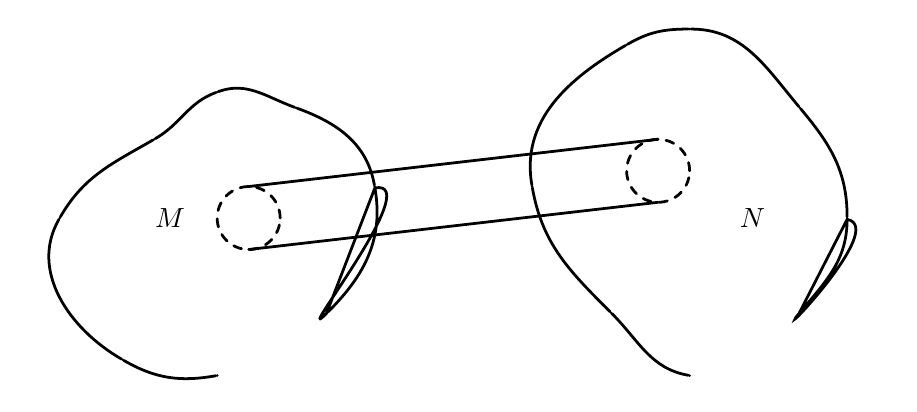
\begin{tikzpicture}[%
    scale=2,
    line width=1pt,
    line cap=round,
]
    \begin{scope}[%
        every node/.style={
            fill=black,
            circle,
            inner sep=0pt,
            outer sep=0pt
        }
    ]
        \node at (0,0) (a) {};
        \node at (-0.6,0.1) (b) {};
        \node at (-1,1) (c) {};
        \node at (-0.4,1.5) (d) {};
        \node at (0, 1.8) (e) {};
        \node at (0.5, 1.7) (f) {};
        \node at (1,1.2) (g) {};
        \node at (0.7,0.4) (h) {};
        \node at (3,0) (a1) {};
        \node at (2.5,0.4) (b1) {};
        \node at (2,1.2) (c1) {};
        \node at (2.6,2.1) (d1) {};
        \node at (3, 2.2) (e1) {};
        \node at (3.7, 1.7) (f1) {};
        \node at (4,1) (g1) {};
        \node at (3.7,0.4) (h1) {};
    \end{scope}
    \node at (-0.3,1) (i) {$M$};
    \node at (3.4,1) (i1) {$N$};
    \draw (a) to [out=-170,in=-30] (b)
              to [out=150,in=-120] (c)
              to [out=60,in=-150] (d)
              to [out=30,in=-160] (e)
              to [out=20,in=160] (f)
              to [out=-20,in=100] (g)
              to [out=-80,in=45] (h)
              to [out=-135,in=10] cycle;
    \draw (a1) to [out=170,in=-45] (b1)
               to [out=135,in=-80] (c1)
               to [out=100,in=-150] (d1)
               to [out=30,in=180] (e1)
               to [out=0,in=130] (f1)
               to [out=-50,in=90] (g1)
               to [out=-90,in=50] (h1)
               to [out=-130,in=-10] cycle;
    \draw[dashed] (0.2,1) circle (0.2);
    \draw[dashed] (2.8,1.3) circle (0.2);
    \draw (0.2,1.2) -- (2.8,1.5);
    \draw (0.2,0.8) -- (2.8,1.1);
\end{tikzpicture}